\newcommand{\threadingSequence}{
Die Daten werden über mehrere Threads übertragen, die Oberen Klassen repräsentieren jeweils einen Thread. An unkritischen Stellen passiert dies per direktem Zugriff oder einem Callback (Abb. \ref{fig:threading_sequence}). Die Daten werden von der Emokit Klasse per Methodenaufruf geholt. Der DataCollector überträgt diese Daten an 1 .. n SignalWindows. Derzeit sind 2 SignalWindows implementiert, diese Zahl lässt sich erweitern. Wenn ein SignalWindow voll ist (128 Werte $\equiv$ 1s) wird ein Callback ausgelöst, der direkt an den FeatureExtractor weitergegeben wird. Die Signal Sequenzen werden dort in eine threadsichere Queue eingefügt und 1 .. n ProcessingChains verarbeiten die Daten. Die Abarbeitung der ProcessingChain ist potentiell aufwändig und ist mit zwei Thread-sicheren Queues umgesetzt. Sollte die Verarbeitung zu lag dauern, könnten weitere ProcessingChains hinzugefügt werden. Der FeatureExtractor reicht diese Daten derzeit auf einer weiteren Queue zur Hauptanwendung, wo die Klassifizierung blockierend angestoßen wird und das Ergebnis zum Ausgabebildschirm geleitet wird. Der FeatureExtractor kann zu einem späteren Zeitpunkt eine Aggregation der Daten vornehmen oder sich um die Verwaltung der ProcessingChains kümmern. Probleme im Testbetrieb macht derzeit die Geschwindigkeit, die Abarbeitung kommt nicht hinterher, da die Testdaten des Emokits zu schnell geliefert werden.
\begin{figure*}
    \makebox[\textwidth][c]{
    	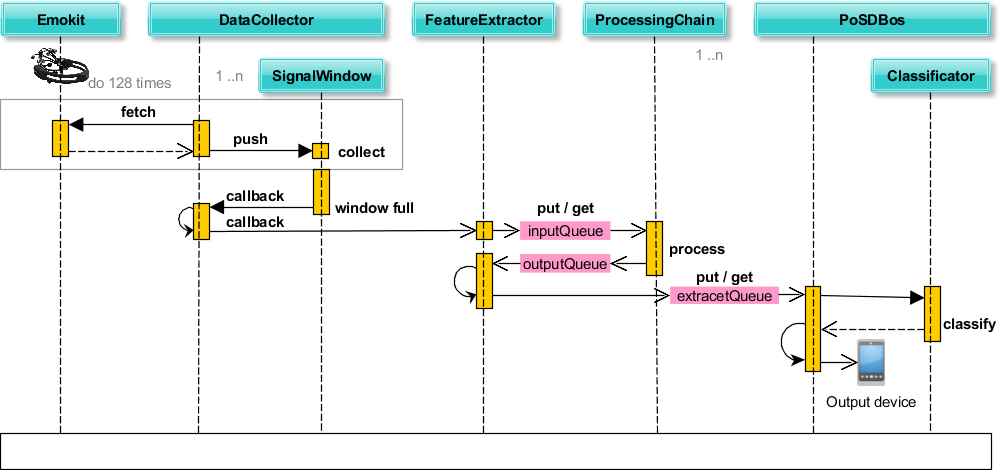
\includegraphics[width=18cm]{threading_sequence}
    }
    \caption[Sequenzdiagramm der Anwendung]{Die Anwedung ist in mehrere Threads unterteilt. SignalWindow und Processing Chain können mehrere Instanzen haben. \label{fig:threading_sequence}}
\end{figure*}
}